\section{Příklad 2}
% Jako parametr zadejte skupinu (A-H)
\druhyZadani{F}

\vspace{1cm}
\large{\textbf{Rešení (Metoda Theveninovy věty):}}
\vspace{0.5cm}

%%% Krok 1
\begin{center}
\textbf{Krok 1} - Překreslíme obvod bez $R_3$. \\
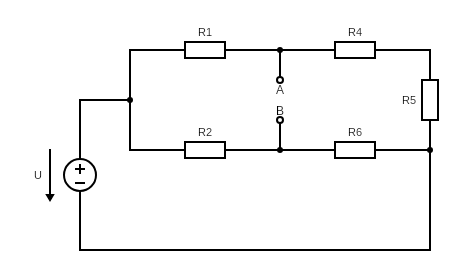
\includegraphics[scale=0.8,keepaspectratio]{fig/Pr2_steps/Pr2_step01.png}
\end{center}

\newpage

%%% Krok 2
\begin{center}
\textbf{Krok 2} - Nahradíme napěťový zdroj zkratem. \\
\hspace{0.8cm}
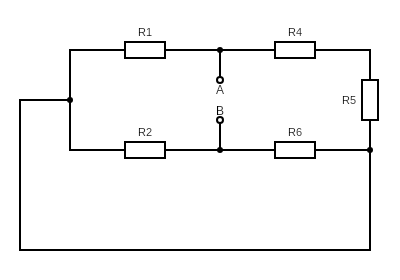
\includegraphics[scale=0.8,keepaspectratio]{fig/Pr2_steps/Pr2_step02.png}
\end{center}
\vspace{0.5cm}

%%% Krok 3
\begin{center}
\textbf{Krok 3} - Vypočítáme  $R_i$. \\
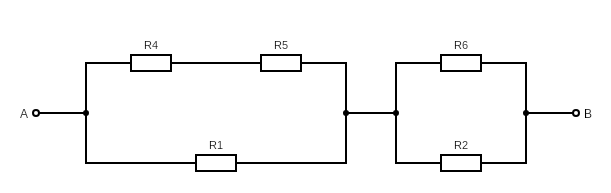
\includegraphics[scale=0.8,keepaspectratio]{fig/Pr2_steps/Pr2_step03.png}
\end{center}
\vspace{-0.3cm}

\begin{gather*}
\newline
R_{45} = R_4 + R_5 = 195 + 650 = 845 \Omega \\\\
\newline
\newline
R_{145} = \frac{R_1 \times R_{45}}{R_1 + R_{45}} = \frac{180 \times 845}{180 + 845} = 148,3902 \Omega \\\\
\newline
\newline
R_{26} = \frac{R_2 \times R_6}{R_2 + R_2} = \frac{350 \times 250}{350 + 250} = 145,8333 \Omega \\\\
\newline
\newline
\boldsymbol{R_i} = R_{26} + R_{145} = 145,8333 + 148,3902 = \boldsymbol{294,2235 \Omega} \\\\
\end{gather*}

\newpage

%%% Krok 4
\begin{center}
\textbf{Krok 4} - Vypočítáme  $U_{R_3}$. \\
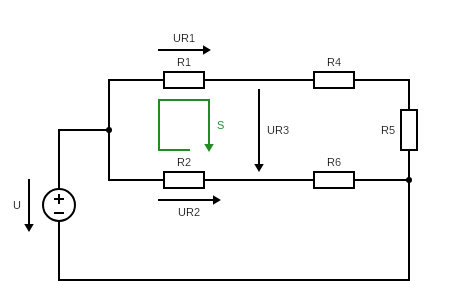
\includegraphics[scale=0.8,keepaspectratio]{fig/Pr2_steps/Pr2_step04.png}
\end{center}
\vspace{-0.3cm}

\begin{gather*}
\newline
U_{R_1} = U \times \frac{R_1}{R_1 + R_4 + R_5} = 130 \times \frac{180}{180 + 195 + 650} = 22,8293 V \\\\
\newline
\newline
U_{R_2} = U \times \frac{R_2}{R_2 + R_6} = 130 \times \frac{350}{350 + 250} = 75,8333 V \\\\
\newline
\newline
S: U = U_{R_1} + U_{R_3} + U_{R_2} = 0\\\\
\newline
\newline
\boldsymbol{U_{R_3}} = U_{R_2} - U_{R_1} = \boldsymbol{53,004 V} \\\\
\end{gather*}

%%% Krok 5
\begin{center}
\textbf{Krok 5} - Vypočítáme  $I_{R_3}$. \\
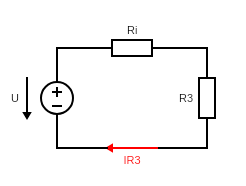
\includegraphics[scale=1,keepaspectratio]{fig/Pr2_steps/Pr2_step05.png}
\end{center}
\vspace{-0.3cm}

\begin{gather*}
\boldsymbol{I_{R_3}} = \frac{U_{R_3}}{R_i + R_3} = \frac{53,004}{294,2235 + 600} = \boldsymbol{0,0593 A} \\\\
\end{gather*}